\chapter{Plot Gallery}
\section{tikz}
下面我们给出zTikZ这部分命令的一些综合绘图案例:
\begin{leftbar}
\noindent 如果你修改了绘图代码,但是发现得到的pdf中的图像并没有改变,那么极有可能是因为
你指定的精度过高,超出了\TeX{}的内存使用限制.(而且由于采用了external库用于缓存,有可能你在编译时并不会抛出
这个错误) 其实比较耗费内存的点主要有3个:
\begin{itemize}
    \item 指定的精度过高, 一般情况下在区间长度$<5$时指定精度为100就已经足够了
    \item 使用了多个\cmd{\ContourPlot}函数,在默认的精度 100下,多个此函数也可能导致内存超出
    \item 最后一点耗时的点就是\cmd{\ShowIntersecion}命令,可以先用Geogebra得到交点后再使用
        \cmd{\ShowPoint}命令进行点的绘制.
    \item 更严重的如果出现了编译错误,请考虑去掉\cmd{\ShadePlot}命令,或在\cmd{\usepackage[external=false]{ztikz}}
        的情况下使用此命令.
\end{itemize}
\end{leftbar}


\subsection{Example 1}
\begin{figure}[!htb]
    \centering
    % show angle 
\tikzset{
    right angle quadrant/.code={
        \pgfmathsetmacro\quadranta{{1,1,-1,-1}[#1-1]}     % Arrays for selecting quadrant
        \pgfmathsetmacro\quadrantb{{1,-1,-1,1}[#1-1]}},
    right angle quadrant=1, % Make sure it is set, even if not called explicitly
    right angle length/.code={\def\rightanglelength{#1}},   % Length of symbol
    right angle length=2ex, % Make sure it is set...
    right angle symbol/.style n args={3}{
        insert path={
            let \p0 = ($(#1)!(#3)!(#2)$) in     % Intersection
                let \p1 = ($(\p0)!\quadranta*\rightanglelength!(#3)$), % Point on base line
                \p2 = ($(\p0)!\quadrantb*\rightanglelength!(#2)$) in % Point on perpendicular line
                let \p3 = ($(\p1)+(\p2)-(\p0)$) in  % Corner point of symbol
            (\p1) -- (\p3) -- (\p2)
        }
    }
}

% main code
\begin{tikzpicture}[scale=.75, >=Latex]
    \ShowGrid[step=1, color=gray, opacity=.5]{(-8, -8); (8, 8)}
    \ShowXYAxis{8}{8}
    % curve
    \ContourPlot[-8:8; -8:8]{x**2/3-y**2/4-1}
    \ContourPlot[-8:8; -8:8][dashed, red]{(x-3.05)**2 + (y-2.18)**2-4.76}
    % points and lines
    \coordinate (A) at (5.69, 6.26);
    \coordinate (B) at (-5, 0);
    \coordinate (C) at (5, 0);
    \coordinate (D) at (3.05, 2.18);
    \draw (A) -- (B) -- (C) -- cycle;
    % angle and 3-lines
    \draw [blue,right angle symbol={A}{1.94,4.06}{D}]; % F
    \draw [blue,right angle symbol={A}{5.21,1.94}{D}]; % E
    \draw [blue,right angle symbol={B}{3.05,0}{D}];    % G
    \draw (D) -- (1.94, 4.06);
    \draw (D) -- (5.21, 1.94);
    \draw (D) -- (3.05, 0);
    \ShowPoint[type=*, color=red]{(A); (B); (C); (D)}[$A$; $F_1$; $F_2$; $o$][below right]
\end{tikzpicture}
    \caption{Parabolic Example}
    \label{fig:1-parabolic}
\end{figure}
\inputminted{latex}{./Example/example_1.tex}
\newpage

\subsection{Example 2}
\begin{figure}[!htb]
    \centering
    \begin{tikzpicture}[yscale=6, xscale=3]
    \ShowGrid{(-2,0); (2,1)}
    % pdf
    \Plot[-2:2][teal]{1/(sqrt(0.2)*sqrt(2*pi))*exp(-(x-0)**2/(2*0.2**2))}
    \Plot[-2:2][orange]{1/(sqrt(0.5)*sqrt(2*pi))*exp(-(x-0)**2/(2*0.5**2))}
    \Plot[-2:2][green]{1/(sqrt(1)*sqrt(2*pi))*exp(-(x-0)**2/(2*1**2))}
    % cdf
    \Plot[-2:2][teal]{0.5*(1+erf((x-0)/(sqrt(0.2)*sqrt(2))))}
    \Plot[-2:2][orange]{0.5*(1+erf((x-0)/(sqrt(0.5)*sqrt(2))))}
    \Plot[-2:2][green]{0.5*(1+erf((x-0)/(sqrt(1)*sqrt(2))))}
    % annotate
    \ShowPoint[radius=0pt]{(-1, 0); (0, 0); (1, 0)}[$\mu-\sigma$; $\mu=0$; $\mu+\sigma$][below]
    \ShowPoint[radius=0pt]{(1, 0.8); (1, 0.6); (1, 0.4)}[
        \textcolor{red}{\rule[1pt]{8pt}{3pt}}\;$\sigma^2=0.2$;
        \textcolor{orange}{\rule[1pt]{8pt}{3pt}}\;$\sigma^2=0.5$;
        \textcolor{green}{\rule[1pt]{8pt}{3pt}}\;$\sigma^2=1$;
    ][right=2em]
    \ShowPoint[radius=0pt]{(-1, 0.8)}[$\displaystyle y = \frac{1}{\sigma\sqrt{2\pi}}\mathrm{Exp}\{-\frac{(x-\mu)^2}{2\sigma^2}\}$]
    \ShowPoint[radius=0pt]{(-1, 0.6)}[$y=\frac12\left(1+\mathrm{Erf}(\frac{x-\mu}{\sigma\sqrt{2}})\right)$]
\end{tikzpicture}
    \caption{Normal-distribution Example}
    \label{fig:2-norm-distribution}
\end{figure}
\inputminted{latex}{./Example/example_2.tex}
\newpage


\subsection{Example 3}
\begin{figure}[!htb]
    \centering
    \begin{tikzpicture}[>=Latex]
    \xAxis[-1][12]
    \yAxis[-1][7]

    \PlotPrecise{plot}{22}
    \Plot[0.75:11][red, thick, opacity=0][type=ball, color=red]{2.5-1/x}

    \PlotPrecise{plot}{22}
    \Plot[0.5:11.5][red, thick, opacity=0][type=ball, color=green]{3+1/x}

    \PlotPrecise{contour}[long]{40}
    \ContourPlot[0:12][dashed]{y-2.5}
    \ContourPlot[0:12][dashed]{y-3}
\end{tikzpicture}
    \caption{Sup and Inf Example}
    \label{fig:3-sup-inf}
\end{figure}
\inputminted{latex}{./Example/example_3.tex}
\newpage


\subsection{Example 4}
\begin{figure}[!htb]
    \centering
    \ExplSyntaxOn
\clist_new:N \l__color_clist
\clist_set:Nn \l__color_clist {red, orange, yellow, green, blue, purple, brown, black}
\newcommand{\colorItem}[1]{\clist_item:Nn \l__color_clist {#1}}
\ExplSyntaxOff
\begin{tikzpicture}[scale=10, >=Latex, font=\scriptsize]
    % plot and annotate
    \node at (.55, 0.15) [left] {$f(x)=\frac{1}{n}\sin(n+5)x$};
    \foreach \i in {6, 7, 8, 9, 10, 11, 12, 13}{
        \Plot[0:pi/3][\colorItem{\fpeval{\i-5}}]{\fpeval{1/\i}*sin(\fpeval{\i+5}*x)}
        \node[color=\colorItem{\fpeval{\i-5}}] at (1, \fpeval{(\i-6)*0.03}) [right] {$n=\i$};
    }
    % axis draw
    \ShowAxis [
        tickStyle=above,    axisColor=gray,
        tickStart=-0.15,    tickEnd=0.18,
        mainStep=0.05,
        mainTickColor=gray, mainTickLabelPosition=left,
        mainTickLength=.5pt,axisRotate=90,
    ]{(-0.18, 0); (0.18, 0)}
    \ShowAxis [
        tickStyle=below,    axisColor=gray,
        tickStart=0,        tickEnd=1.22,
        mainStep=\fpeval{3.1415926/18},
        mainTickColor=gray, subTickLength=0pt, 
        mainTickLength=.5pt, 
        mainTickLabel={\fpeval{\CurrentFp/(3.1415926/18)*10}$^\circ$}
    ]{(0, 0); (1.25, -0)}
\end{tikzpicture}
    \caption{Loop Plot Example}
    \label{fig:4-loop-to-plot-function}
\end{figure}
\inputminted{latex}{./Example/example_4.tex}
\newpage

\subsection{Example 5}
\begin{figure}[!htb]
    \centering
    \begin{tikzpicture}[>=Latex]
    % draw axis
    \xAxis[0][10]
    \yAxis[-3.25][3.25]
    % plot ucntion and  generate discrete points
    \Plot[0:10]{2*sqrt(x)*cos(log(x))*sin(x)}
    \PlotPrecise{plot}{40}
    \Plot[0:10][opacity=0][type=*, color=red]{2*sqrt(x)*cos(log(x))*sin(x)}
    % bar plot
    \BarPlot[x][fill=orange!35!white, bar width=\fpeval{10/40}cm, opacity=.75, very thin, draw=orange]{\gnudata{2}}
\end{tikzpicture}
    \caption{Darboux Example}
    \label{fig:5-darboux-function}
\end{figure}
\inputminted{latex}{./Example/example_5.tex}
\newpage


\subsection{Example 6}
\begin{figure}[!htb]
    \centering
    \begin{tikzpicture}[>=Latex]
    % grid and axis
    \ShowGrid[step=1, color=gray, opacity=.5]{(0, 0); (10, 10)}
    \xAxis[-1][10]      \yAxis[-1][10]
    % plot and points
    \Plot[0:10][red, jump mark right, very thick, xshift=2pt][type=*, opacity=0]{floor(x)}
    \Plot[0:10][dashed, blue]{x}
    \Plot[1:10][dashed, orange]{x-1}
    \PlotPrecise{plot}{11}
    \Plot[0:10][opacity=0, jump mark right][type=o, color=blue]{x}
    \PlotPrecise{plot}{11}
    \Plot[0:10][opacity=0, jump mark right][type=*, color=red]{x-1}
    \ShowPoint[opacity=0]{(2, 9); (2, 8); (2, 7)}[$y=\lfloor x\rfloor$; $y=x$; $y=x-1$][right]
\end{tikzpicture}
    \caption{Stairs Function Example}
    \label{fig:6-stairs-function}
\end{figure}
\inputminted{latex}{./Example/example_6.tex}
\newpage


\subsection{Example 7}
\begin{figure}[!htb]
    \centering
    \input{./Example/example_7.tex}
    \caption{Functions and Points Example}
    \label{fig:7-points-function}
\end{figure}
\inputminted{latex}{./Example/example_7.tex}
\newpage


\subsection{Example 8}
\begin{figure}[!htb]
    \centering
    \begin{tikzpicture}[font=\small, >=Latex, scale=.65]
    %% ==> ztikz draw grid(coordinates)
    \ShowGrid{(-8, -8); (8, 8)}
    \ShowPoint{(0, 0)}[$O=(0, 0)$][below right]
    \ShowAxis {(0, -8); (0, 8)}
    \ShowAxis {(-8, 0); (8, 0)}

    % contour plot
    \PlotPrecise{contour}[long]{10}
    \ContourPlot[-8:8; -8:8][thick, red]{x+6}
    \ContourPlot[-8:8; -8:8][thick, red]{y+6}
    \ContourPlot[-8:8; -8:8][thick, blue]{y-6}
    \ContourPlot[-8:8; -8:8][thick, blue]{x-6}
    \PlotPrecise{contour}[long]{100}
    \ContourPlot[-4:4][green]{x**2/9+y**2/4-1}
    \ContourPlot[-7:7; -7:7][teal]{sin(x**2+y**2)-exp(-x*y)}

    % polar plot
    \begin{scope}[xshift=4cm, yshift=-5cm]
        \PolarPlot[0:10*pi][orange]{0.1*t}
    \end{scope}
    \begin{scope}[xshift=-4cm, yshift=5cm]
        \PolarPlot{2*(1-sin(t))}
        \fill[gray, opacity=.5] plot file {\gnudata{8}};
    \end{scope}

    % node annotate
    \ShowPoint[opacity=0]{(-4, 3); (4, 5); (5, -5); (3, -1)}
        [$\rho=2(1-\sin\theta)$; $\sin(x^2+y^2)-\exp(-xy)=0$; $\rho=0.1\theta$; $\frac{x^2}{9} + \frac{y^2}{4}=1$]
\end{tikzpicture}
    \caption{Polar and Contour Example}
    \label{fig:polar-contour-plot}
\end{figure}
\inputminted{latex}{./Example/example_8.tex}
\newpage


\subsection{Example 9}
\begin{figure}[!htb]
    \centering
    \begin{tikzpicture}[>=Latex, font=\small, scale=1.5]
    % basic
    \clip (-6, -1) rectangle (3, 6);
    \ShowAxis{(-8, 0); (3, 0)}      \ShowAxis{(0, -1.5); (0, 6)}
    % functions
    \Plot[-8:5][red]                {exp(x)}
    \Plot[-8:5][blue]               {exp(1)/4*(x+1)**2}
    \Plot[-8:5][green]              {exp(1)*x + (x-1)**2}
    \Plot[-8:5][purple]             {x**2 + 1}
    \Plot[-8:0.95][gray]            {1/(1-x)}
    \Plot[-8:1.95][orange]          {(2+x)/(2-x)}
    \Plot[-8:5]                     {x+1}
    \Plot[-8:8]                     {exp(1)*x}
    \ContourPlot[0:2;-6:6][dashed]  {x-1}
    % points
    \ShowPoint[color=red, radius=1pt]{(-1, 0); (0, 1); (1, 2.71828)}[$A$; $B$; $C$][above left]
\end{tikzpicture}
    \caption{Exp Functions Example}
    \label{fig:9-exp-functions}
\end{figure}
\inputminted{latex}{./Example/example_9.tex}
\newpage



\subsection{Example 10}
\begin{figure}[!htb]
    \centering
    \input{./Example/example_10.tex}
    \caption{Log Functions Example}
    \label{fig:10-log-function}
\end{figure}
\inputminted{latex}{./Example/example_10.tex}
\newpage
